\documentclass[11pt]{article}
\usepackage[top=1in, bottom=1in,right=1in,left=1in]{geometry}                % See geometry.pdf to learn the layout options. There are lots.
\geometry{letterpaper}                   % ... or a4paper or a5paper or ... 
%\geometry{landscape}                % Activate for for rotated page geometry
%\usepackage[parfill]{parskip}    % Activate to begin paragraphs with an empty line rather than an indent
\usepackage{graphicx}
\usepackage{amssymb}
\usepackage{amsmath}
\usepackage{amsthm} %pour les newtheorem
\usepackage{epstopdf}
\usepackage{xspace}
\usepackage{relsize}
\usepackage[numbers]{natbib}
\usepackage[colorinlistoftodos]{todonotes}

%\usepackage{subfig} %Subfigures
\usepackage{subcaption} %Subfigures

\usepackage{tikz}
\usepackage{amsmath}
\usepackage{ifthen}
\usepackage{relsize}
\usetikzlibrary{positioning}
\usetikzlibrary{matrix}
\usetikzlibrary{calc}
\usetikzlibrary{shapes}
\usetikzlibrary{arrows}
\usetikzlibrary{fit}
\usetikzlibrary{decorations}
\usetikzlibrary{snakes}
\pgfdeclarelayer{background}
\pgfdeclarelayer{backbackground}
\pgfdeclarelayer{foreground}
\pgfsetlayers{backbackground,background,main,foreground}




\newcommand{\ourprog}{\texttt{RNA-MoIP}\xspace} 

\usepackage[applemac]{inputenc} %for the encoding 


\newcommand{\RNAmutants}{\texttt{RNAmutants}\xspace}
\newcommand{\RNApyro}{\texttt{RNApyro}\xspace}

\newcommand{\red}[1]{{\color{red}#1}}
\newcommand{\farna}{\texttt{FARNA}\xspace}
\newcommand{\mcfoldmcsym}{\texttt{MC-Pipeline}\xspace}
\newcommand{\mcfold}{\texttt{MC-Fold}\xspace}
\newcommand{\mcsym}{\texttt{MC-Sym}\xspace}
\newcommand{\nast}{\texttt{NAST}\xspace}
\newcommand{\ifoldrna}{\texttt{iFoldRNA}\xspace}
\newcommand{\rnafold}{\texttt{RNAfold}\xspace}
\newcommand{\rnasubopt}{\texttt{RNAsubopt}\xspace}
\newcommand{\rnawolf}{\texttt{RNAwolf}\xspace}
\newcommand{\rnastructure}{\texttt{RNAstructure}\xspace}
\newcommand{\contrafold}{\texttt{contrafold}\xspace}
\newcommand{\unafold}{\texttt{unafold}\xspace}
\newcommand{\rnadd}{\texttt{RNA2D3D}\xspace}
\newcommand{\assemble}{\texttt{assemble}\xspace}
\newcommand{\fred}{\texttt{FR3D}\xspace}
\newcommand{\rnajunction}{\texttt{RNAjunction}\xspace}
\newcommand{\rnamotif}{\texttt{RNAmotif}\xspace}
\newcommand{\treefolder}{\texttt{TreeFolder}\xspace}
\newcommand{\barnacle}{\texttt{BARNACLE}\xspace}
\newcommand{\contextfold}{\texttt{contextfold}\xspace}
%\newcommand{\citep}{\cite}
\newcommand{\Z}[3]{\mathcal{Z}_{\substack{(#1)\\ [#3]}}^{#2}}
\newcommand{\Y}[3]{\mathcal{Y}_{\substack{(#1)\\ [#3]}}^{#2}}
\newcommand{\B}{\mathcal{B}}
\newcommand{\Kron}{\delta}
\newcommand{\ub}{\bullet}

\newcommand{\Ab}{{\sf{A}}}
\newcommand{\Cb}{{\sf{C}}}
\newcommand{\Gb}{{\sf{G}}}
\newcommand{\Ub}{{\sf{U}}}

%\title{An inside-outside algorithms for mutant RNAs with applications to error detections in structured RNAs}
\title{A linear inside-outside algorithm for correcting sequencing errors in structured RNA}
\author{Vladimir Reinharz, Yann Ponty$^{*}$, J\'er\^{o}me Waldisp\"{u}hl$^*$}
\date{}


%Last thing before BEGIN DOC for links to appear in pdf

%  \usepackage{hyperref}
%  \hypersetup{colorlinks}
%              citecolor=black,
%              filecolor=black%
%              linkcolor=black%
%              urlcolor=black%
%              pdftex}

\begin{document}
\maketitle
%\section{}
%\subsection{}
\begin{abstract}
Analysis of the sequence-structure relationship in RNA molecules are essential to evolutionary studies but also to 
concrete applications such as error-correction methodologies in sequencing technologies. The prohibitive sizes of the
mutational and conformational landscapes combined with the volume of data to proceed require efficient algorithms 
to compute sequence-structure properties. More specifically, here we aim to calculate which mutations increase the most the 
likelihood of a sequence to a given structure and RNA family.\\
In this paper, we introduce \RNApyro, an efficient linear-time and space inside-outside algorithm that computes exact mutational
probabilities under secondary structure and evolutionary constraints given as a multiple sequence alignment with a consensus structure.
We develop a scoring scheme combining classical stacking base pair energies to novel isostericity scales, and apply our techniques
to correct point-wise errors in 5s rRNA sequences. Our results suggest that \RNApyro is a promising algorithm to complement existing
tools in the NGS error-correction pipeline. 

\noindent
\textbf{Key words:} RNA, mutations, secondary structure
\end{abstract}

\newpage

%!TEX root = main_RECOMB.tex
\section{Introduction}
\label{sec:introduction}

Ribonucleic acids (RNAs) are found in every living organisms and exhibit a broad range of functions, from catalyzing
chemical reactions as the RNase P or the group II introns, hybridizing  messenger RNA to regulate gene expression,
to ribosomal RNA (rRNA) synthesizing proteins. Those functions  require specific structures,  encoded in their nucleotide
sequence. Although the functions, and thus the structures, need to be preserved through various organisms, the sequences
can greatly differ from one organism to another. This sequence diversity coupled with the structural conservation is a fundamental
asset for evolutionary studies. To this end, algorithms to analyze the relationship between RNA mutants and structures are required.

For half a century, biological molecules have been studied as a proxy to understand evolution~\cite{Zuckerkandl1965}, and due
to their fundamental functions and remarkably conserved structures, rRNAs have always been a prime candidate for phylogenetic
studies~\cite{Olsen1986, Olsen1993}. In recent years, studies as the \emph{Human Microbiome Project}~\cite{Turnbaugh2007} benefited
of new technologies such as the NGS techniques to sequence as many new organisms as possible and extract an unprecedented flow of new information. 
Nonetheless, these high-throughput techniques typically have high error rates that make their applications to metagenomics (a.k.a. environmental
genomics) studies challenging. For instance, pyrosequencing as implemented by Roche's 454 produces may have a error rate raising up to 10\%.
Because there is no cloning step, resequencing to increase accuracy is not possible and it is therefore vital to disentangle noise from true sequence
diversity in this type of data \cite{Quince:2009uq}. Errors can be significantly reduced  when large multiple sequence alignments with close homologs
are available, but in studies of new or not well known organisms, such information is rather sparse. In particular, it is common to is not enough  similarity to 
differentiate between the sequencing errors and the natural polymorphisms that we want to observe, often inflating the diversity estimates~\cite{Kunin2010}.
A few techniques have been developed to remedy to this problem~\cite{Quinlan2008,Medvedev2011} but they do not take
into account all the available information. It is therefore essential to develop methods that can exploit any type of signal available to correct errors.  

In this paper, we introduce \RNApyro, a novel algorithm to that enable us to calculate precisely mutational probabilities in RNA sequences with a
conserved consensus secondary structure. We show how our techniques can exploit the structural information embedded in physics-based energy models, 
covariance models and isostericity scales to identify and correct point-wise errors in RNA molecules with conserved secondary structure. In particular, we 
hypothesize that  conserved consensus secondary structures combined with sequence profiles  provide an information that allow us to identify and fix sequencing errors.

Here, we expand the range of algorithmic techniques previously introduced with \RNAmutants~\cite{Waldispuhl2008}.
Instead of exploring the full conformational landscape and sample mutants, we develop an inside-outside algorithm that enables us
to explore the complete mutational landscape with a \emph{fixed} secondary structure and to calculate exactly mutational probability values. In addition
to a gain into the numerical precision, this strategy allows us to drastically reduce the computational complexity ($\mathcal{O}(n^3 \cdot m^2)$ for the
original version of  \RNAmutants to $\mathcal{O}(n \cdot m^2)$ for \RNApyro, where $n$ is the size of the sequence and $m$ the number of mutations).

We design a new scoring scheme combining nearest-neighbor models \cite{Turner2010} to isostericity metrics \cite{Stombaugh2009}.
Classical approaches use a Boltzmann distribution whose weights are estimated using a nearest-neighbour energy model~\cite{Turner2010}. However, the
latter only accounts for  canonical and wobble, base pairs. As was shown by Leontis and Westhof~\cite{Leontis2001},
the diversity of base pairs observed in tertiary structures is much larger, albeit their energetic contribution remains unknown. To quantify geometrical discrepancies, 
an isostericity distance has been designed \cite{Stombaugh2009}, increasing as two base pairs geometrically differ from each other in space. Therefore, we 
incorporate these scores in the Boltzmann weights used by \RNApyro.
 
We illustrate and benchmark our techniques for point-wise error corrections on the 5S ribosomal RNA. We choose the latter since it has been extensively
used for phylogenetic reconstructions~\cite{Hori1987} and its sequence has been recovered for over 712 species (in the Rfam seed alignment with id
\texttt{RF00001}). Using a leave one out strategy, we perform random distributed mutations on a sequence. While our methodology is restricted to the correction of 
point-wise error in structured regions (i.e. with base pairs), we show that \texttt{RNApyro} can successfully extract a signal that can be used to reconstruct the 
original sequence with an excellent accuracy. This suggests that \RNApyro is a promising algorithm to complement existing tools in the NGS error-correction 
pipeline.

The algorithm and the scoring scheme are presented in Sec.~\ref{sec:methods}. Details of the implementation and benchmarks are in Sec.~\ref{sec:results}. 
Finally, we discuss future developments and applications in Sec.~\ref{sec:conclusion}.

%!TEX root = main_RECOMB.tex
\section{Methods}
\label{sec:methods}

\newcommand{\PE}[1]{E(#1)}
\newcommand{\EI}{\text{EI}}
\newcommand{\ES}{\text{ES}}
\newcommand{\ISO}{\text{ISO}}
We introduce a probabilistic model, which aims at capturing both the stability of the folded RNA and its ability to adopt a predefined 3D conformation.
To that purpose, a Boltzmann weighted distribution is used, based on a pseudo-energy function $\PE{\cdot}$ which includes contributions for both the free-energy and its putative isostericity towards a multiple sequence alignment. In this model, the probability that the nucleotide at a given position needs to be mutated (i.e. corresponds to a sequencing error) can be computed using a variant of the \emph{Inside-Outside algorithm}~\cite{Lari1990}.

\subsection{Probabilistic model}
Let $\Omega$ be an gap-free RNA alignment sequence, $S$ its associated secondary structure, 
then any sequence $s$ is assigned a probability proportional to its Boltzmann factor
\begin{align*}
  \mathcal{B}(s) &= e^\frac{-\PE{s}}{RT}, &&\text{with}&\PE{s}&:=\alpha\cdot\ES(s,S)+(1-\alpha)\cdot\EI(s,S,\Omega),
\end{align*}
where $R$ is the Boltzmann constant, $T$ the temperature in Kelvin, $\ES(s)$ and $\EI(s,S,\Omega)$ 
are the free-energy and isostericity contributions respectively (further described below), and $\alpha\in[0,1]$ is an arbitrary parameter that sets the relative weight for both contributions.

\subsubsection{Energy contribution}
The free-energy contribution in our pseudo-energy model corresponds to an additive stacking-pairs model, taking values from the Turner 2004 model retrieved from the NNDB~\cite{Turner2010}. Given a candidate sequence $s$ for a secondary structure $S$, the free-energy of $S$ on $s$ is given by
\begin{align*}
  \ES(s,S) = \sum_{\substack{(i,j)\to (i',j')\in S\\ \text{stacking pairs}}}\ES^{\beta}_{s_is_j\to s_{i'}s_{j'}} 
\end{align*}
where $\ES^{\beta}_{ab\to a'b'}$ is set to $0$ if $ab=\varnothing$ (no base-pair to stack onto), the tabulated free-energy of stacking pairs $(ab)/(a'b')$ in the Turner model if available, or $\beta\in[0,\infty]$ for non-Watson-Crick/Wobble entries (i.e. not in $\{\Gb\Ub,\Ub\Gb,\Cb\Gb,\Gb\Cb, \Ab\Ub\text{ or }\Ub\Ab\}$). This latter parameter allows to choose whether to simply penalize invalid base pairs, or forbid them altogether ($\beta = \infty$).
The loss of precision due to this simplification of the Turner model remains reasonable since the targeted secondary structure is fixed 
(e.g. multiloops do not account for base-specific contributions). Furthermore, it greatly eases the design and implementation of dynamic-programming equations. 
\subsubsection{Isostericity contribution}
The concept of isostericity score~\cite{Stombaugh2009} is based on the geometric discrepancy (superimposability) of two base-pairs, using individual additive contributions computed by Stombaugh~\emph{et al}~\cite{Stombaugh2009}. Let $s$ be a candidate sequence for a secondary structure $S$, given in the context of a gap-free RNA alignment $\Omega$,  we define the contribution of the isostericity to the pseudo-energy as
\begin{align*}
  \ES(s,S,\Omega) &= \sum_{\substack{(i,j)\in S\\ \text{pairs}}}\EI^{\Omega}_{(i,j),s_i s_j}, & \text{where}&& 	\EI^{\Omega}_{(i,j),ab}:=
	\frac{
		\sum_{s'\in\Omega}
			\text{\ISO}((s_i',s_j'),(a,b))}
%-		\left(			\text{\ISO}((s_i',s_j'),(s_i,s_j))				\right)	
{		
		|\Omega|
	}
\end{align*}
is the average isostericity of a base-pair in the candidate sequence, compared with the reference alignment.
The $\ISO$ function uses the {Watson-Crick/Watson-Crick} cis isostericity matrix computed by Stombaugh~\emph{et al}~\cite{Stombaugh2009}. Isostericity scores range between $0$ and $9.7$, with $0$ being assigned to a perfect isostericity, and a penalty of $10$ is used for missing entries.
The isostericity contribution will favor exponentially sequences that are likely to adopt a similar local conformation as the sequences contained in the alignment.

\subsection{Mutational profile of sequences}


Let $s$ be an RNA sequence, $S$ a reference structure, and $m\geq 0$ a desired number of mutations. 
We are interested in  the probability that a given position contains a specific nucleotide, over all sequences having at most $m$ mutations from $s$
%  under the SCFG derivation $S$ 
(formally $\mathbb{P}(s_i = x\mid s,\Omega, S,m)$). 
We define a variant of the
 \emph{Inside-Outside algorithm}~\cite{Lari1990}, allowing us to obtain the
 desired probability,  the two  functions
$\mathcal{Z}_*^*$ and $\mathcal{Y}_*^*$. 

The former, defined in Equations~\eqref{eq:Z_in} and~\eqref{eq:Z_rec}, is analogous to the \emph{inside} algorithm.
It is the partition function, i.e. the sum of Boltzmann factors, over all sequences within $[i,j]$, 
knowing that position $i-1$ is composed of nucleotide $a$ (resp. $j+1$ is $b$), within 
$m$ mutations of $s$. The latter, defined by Equations~\eqref{eq:Y_in} and~\eqref{eq:Y_rec},
 computes the \emph{outside} algorithm, i.e.  
the partition function over sequences within $m$ mutations of $s$, restricted to two intervals $[0,i]\cup[j,n-1]$, and 
knowing  that position $i+1$ is composed of $a$ (resp. $j-1$ is $b$). A suitable combination of these terms, given in Equation~\eqref{eq:combine}, gives the total weight, and in turn the probability, of seeing a specific base at a given position.

%Drawing a parallel with stochastic context-free grammars (SCFG), for which the inside-outside algorithm was introduced, the set of sequences can be seen as the language of words having length $n$, generated from a stochastic context-free grammar.
%These rules would limit the number of mutations (i.e. )
% $S$ can be considered as constraining weighing on the shape of parse trees the derivations in a classic 
% of the {SCFG} generating  all  secondary structures of length  $|s|$. 





\subsubsection{Definitions}
Let $B:=\left\{\Ab,\Cb,\Gb,\Ub\right\}$ be the set of nucleotides.
Given $s\in B^n$ an RNA sequence, let $s_i$ be the nucleotide at position $i$. Let $\Omega$ be a set of un-gapped RNA sequences of
length $n$, and $S$ a secondary structure without pseudoknots. 
Formally, if $(i,j)$ and $(k,l)$ are base pairs in $S$, there is no overlapping extremities
 $\{i,j\}\cap \{k,l\}=\varnothing$ and either the intersection is empty 
 ($[i,j]\cap[k,l]=\varnothing$) or one is included in the other ($[k,l]\subset[i,j]$ or 
 $[i,j]\subset[k,l])$. 

Let us then remind the Hamming distance function $\delta: B^*\times B^* \to \mathbb{N}^+$, which takes two sequences $s'$ and $s''$ as input, $|s'|=|s''|$, and returns the number of differing positions.
Finally, let us denote by $E_{(i,j),ab \to ab'}^{\Omega,\beta}$ the local contribution of a base-pair $(i,j)$ to the pseudo-energy, such that
\begin{equation}
  E_{(i,j),ab \to a'b'}^{\Omega,\beta}  = \alpha \cdot\ES^\beta_{a b \to a' b'}+(1-\alpha)\cdot\EI^{\Omega}_{(i,j),a'b'}.
\end{equation}


\subsubsection{Inside}
\begin{figure}
\resizebox{\textwidth}{!}{
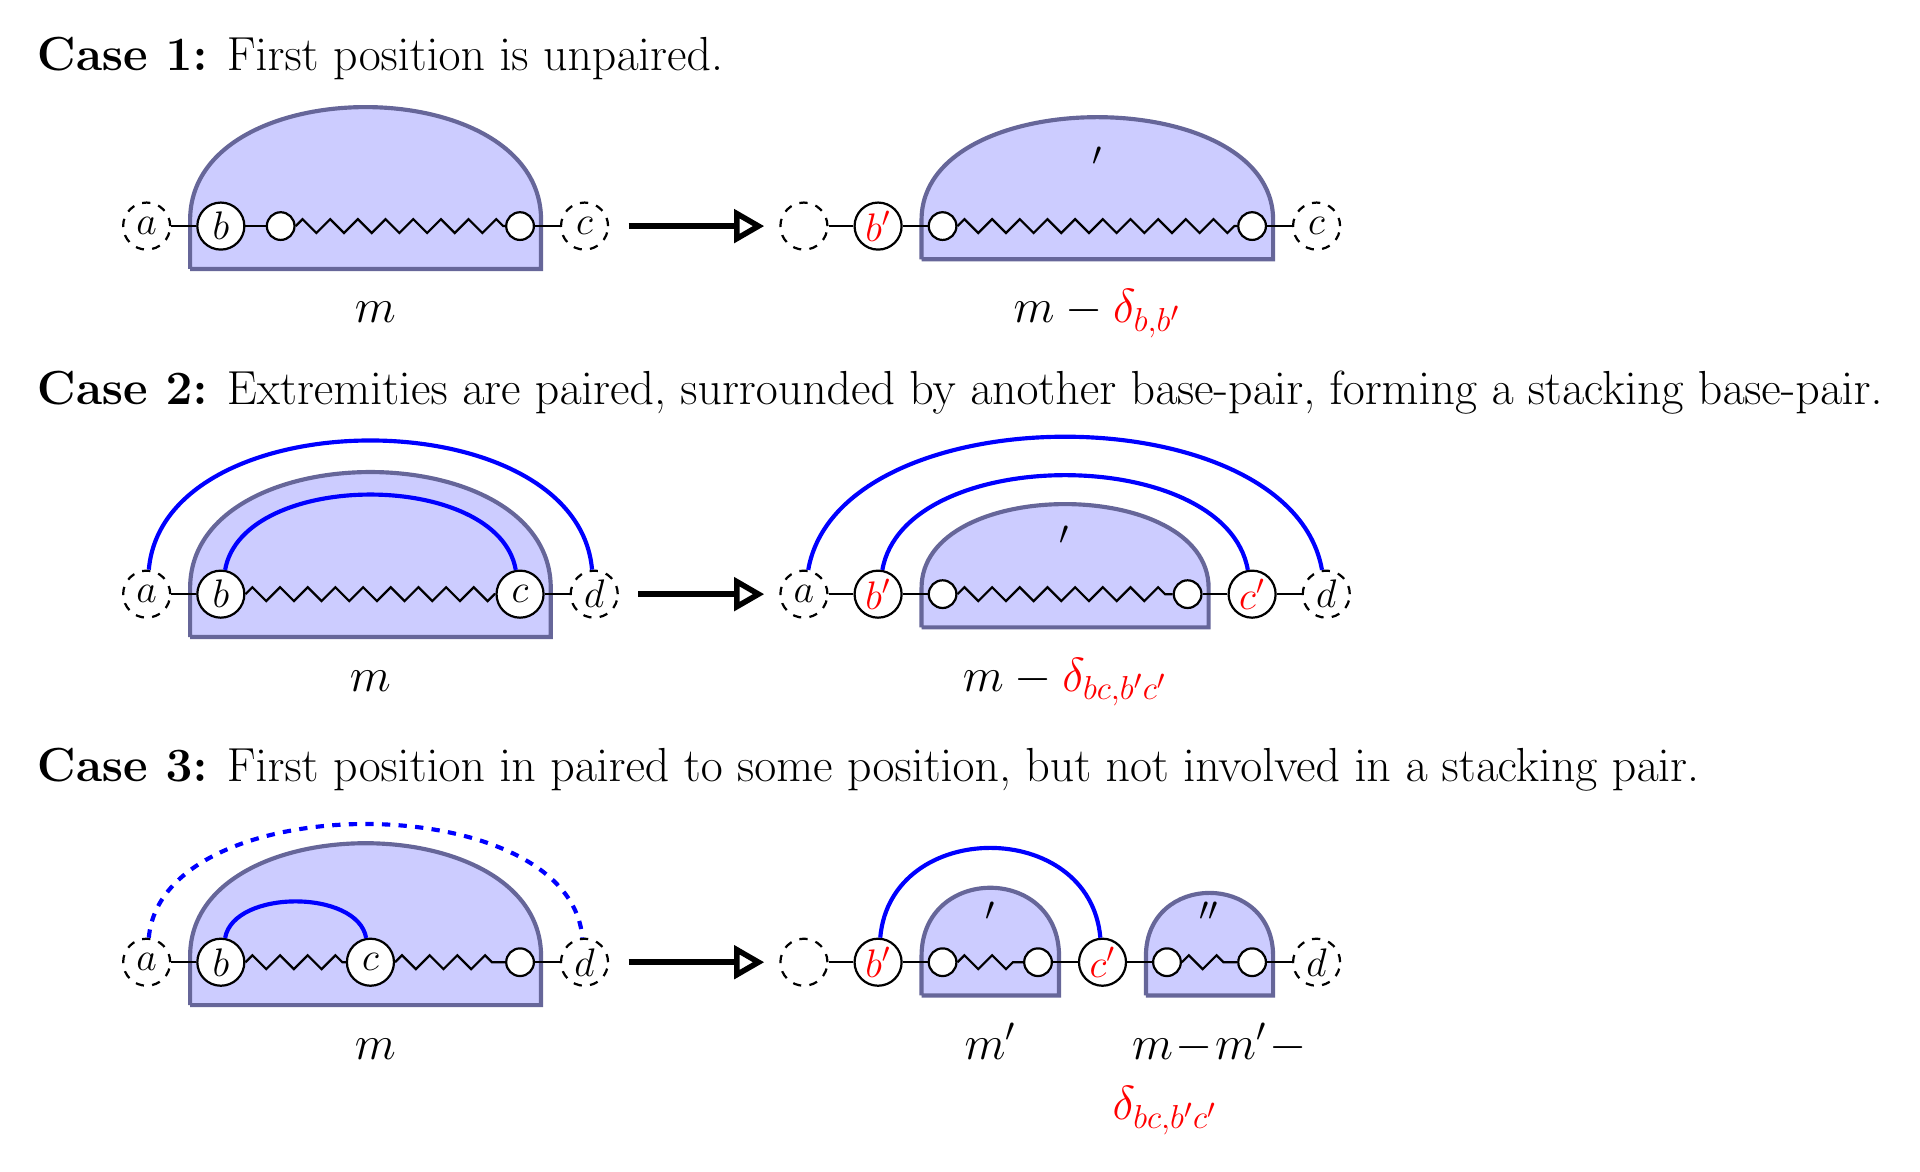
\begin{tikzpicture}[scale=.95]

  \newcommand{\BSep}{9pt}
  \newcommand{\HSep}{250pt}
  \newcommand{\VSepUp}{140pt}
  \newcommand{\VSepDown}{-140pt}
  \newcommand{\LabSepA}{63pt}
  \newcommand{\LabSepB}{75pt}
  \newcommand{\LabSepC}{72pt}
 
  \tikzstyle{base}=[circle,draw,thick,inner sep=0,minimum width=17pt,fill=white,,font={\relsize{+2}}]
  \tikzstyle{basesmall}=[circle,draw,thick,inner sep=0,minimum width=10pt,fill=white]
  \tikzstyle{basephantom}=[base,dashed,font=\relsize{+2}]
  \tikzstyle{linez}=[draw,snake=zigzag, segment aspect=.2,%
line after snake=0pt, 
        segment length=10pt,thick]
  \tikzstyle{lined}=[linez,draw,snake=none,thick]
  \tikzstyle{line}=[linez,draw,snake=none,thick]
  \tikzstyle{bp}=[in=95,out=85,draw,line width=1.5pt,blue,looseness=1]
  \tikzstyle{block}=[trapezium,trapezium angle=33, fill=blue!20, draw=blue!20!gray,line width=1.5pt, inner sep=0]
  \tikzstyle{lbl}=[inner sep=0]
  \tikzstyle{arr}=[line width=1.5pt,-open triangle 60,line width=2pt]
  \tikzstyle{caption}=[%fill=gray!20,draw=gray!60,thick,inner sep=4pt,rounded corners=6pt,
font=\relsize{+3},anchor=north west,xshift=-70pt]
  \tikzstyle{prob}=[fill=none,above=5pt,font=\relsize{+4},draw=none]
  \tikzstyle{cap2}=[fill=none,above=12pt,font=\relsize{+3}]





%% Inside part %%%%%%%%%%
{
%% Unpaired case %%%%%%%%%%

\begin{scope}[yshift=\VSepUp]
  \node[base] (a-1) at (0,0) {$b$};
  \node[basesmall] (a-1b) at (.8,0) {};
  \node[basesmall] (a-2) at (4,0) {};
  \node[left=\BSep of a-1, basephantom] (a-0) {$a$};
  \node[right=\BSep of a-2, basephantom] (a-3) {$c$}; 
  \node[right=0 of a-3] (x1) {};


  \path[lined] (a-1) --  (a-1b);
  \path[linez] (a-1b) --  (a-2);
  \path[lined] (a-0) -- (a-1);
  \path[lined] (a-2) -- (a-3);
  \node[lbl,below=3pt of a-1] (c1) {};
  \node[lbl,below=3pt of a-2] (c2) {};
  \path (a-1) --  node (xx1) {\phantom{xx3}} (a-2);

  \path[draw=none] (a-1) -- node[cap2] (s1) {$\Struct$}  (a-2);

  \begin{pgfonlayer}{background}
  \node[rectangle,inner sep=2pt,draw,fit=(a-1.west)(a-2.east) (c1) (c2)] (r1) {};
  \path[block]   (r1.south west) to (r1.south east) to (r1.north east) to[out=90,in=90,looseness=1.1] (r1.north west) to (r1.south west) ;
  \end{pgfonlayer}{background}
\end{scope}
\node[above= \LabSepA of a-1, caption] {{\bf Case 1:} First position is unpaired.};

\begin{scope}[xshift=\HSep,yshift=\VSepUp]
  \node[base] (a-1) at (0,0) {\color{red}$b'$};
  \node[basesmall,right=\BSep of a-1] (a-1b)  {};
  \node[basesmall] (a-2) at (5,0) {};
  \node[left=\BSep of a-1, basephantom] (a-0) {}; 
  \node[right=\BSep of a-2, basephantom] (a-3) {$c$};
  \path[linez] (a-1b) -- node (xy1) {} node[cap2] {$\Struct'$}  (a-2);
  \path[line] (a-1) -- (a-1b);
  \path[lined] (a-0) -- (a-1);
  \path[lined] (a-2) -- (a-3);
  \node[below=3pt of a-1b, inner sep=0] (c1) {};
  \node[below=3pt of a-2, inner sep=0] (c2) {};

  \node[xshift=-2pt] at (a-0.west) (y1) {};

\begin{pgfonlayer}{background}
  \node[rectangle,inner sep=2pt,draw,fit=(a-1b.west)(a-2.east) (c1) (c2)] (r1) {};
  \path[block]   (r1.south west) to  (r1.south east) to (r1.north east) to[out=90,in=90,looseness=1] (r1.north west) to (r1.south west) ;
  \end{pgfonlayer}{background}

\end{scope}

  \path (x1) edge[arr]    (y1);


%%%Stacking case %%%
\begin{scope}[yshift=0]
  \node[base] (a-1) at (0,0) {$b$};
  \node[base] (a-2) at (4,0) {$c$};


  \node[left=\BSep of a-1, basephantom] (a-0) {$a$};
  \node[right=\BSep of a-2, basephantom] (a-3) {$d$};
  \node[right=0 of a-3] (x2) {};

  \path[linez] (a-1) -- node (xx2) {} node[cap2,yshift=-4pt] (s2) {$\Struct$}  (a-2);

  \path[lined] (a-0) -- (a-1);
  \path[lined] (a-2) -- (a-3);
  \node[lbl,below=3pt of a-1] (c1) {};
  \node[lbl,below=3pt of a-2] (c2){};

  \draw[bp,looseness=1]  (a-0) to (a-3);
  \draw[bp,out=80,in=100,looseness=.9]  (a-1) to (a-2);
  \node[xshift=-2pt] at (a-0.west) (y3) {};

\begin{pgfonlayer}{background}
  \node[rectangle,inner sep=2pt,draw,fit=(a-1.west)(a-2.east) (c1) (c2)] (r1) {};
  \path[block]   (r1.south west) to   (r1.south east) to (r1.north east) to[out=90,in=90,looseness=1.1] (r1.north west) to (r1.south west) ;
  \end{pgfonlayer}{background}
\end{scope}
\node[above= \LabSepB of a-1, caption] {{\bf Case 2:} Extremities are paired, surrounded by another base-pair, forming a stacking base-pair.};

\begin{scope}[xshift=\HSep,yshift=00pt]
  \node[base] (a-1) at (0,0) {\color{red}$b'$};
  \node[base] (a-2) at (5,0) {\color{red}$c'$};

  \node[basesmall,right=\BSep of a-1] (a-1b) {};
  \node[basesmall,left=\BSep of a-2] (a-2b)  {};

  \node[left=\BSep of a-1, basephantom] (a-0) {$a$};
  \node[right=\BSep of a-2, basephantom] (a-3) {$d$};

  \path[linez] (a-1b) -- node (xy2) {}  node[cap2,yshift=-4pt]  {$\Struct'$}  (a-2b);

  \path[line] (a-1) -- (a-1b);
  \path[line] (a-2) -- (a-2b);
  \path[lined] (a-0) -- (a-1);
  \path[lined] (a-2) -- (a-3);
  \node[lbl,below=3pt of a-1b] (c1) {};
  \node[lbl,below=3pt of a-2b] (c2){};

  \draw[bp,out=80,in=100,looseness=.9]  (a-1) to (a-2);
  \draw[bp,out=80,in=100,looseness=.9]  (a-0) to (a-3);
  \node[xshift=-2pt] at (a-0.west) (y2) {};

\begin{pgfonlayer}{background}
  \node[rectangle,inner sep=2pt,draw,fit=(a-1b.west)(a-2b.east) (c1) (c2)] (r1) {};
  \path[block]   (r1.south west) to  (r1.south east) to (r1.north east) to[out=90,in=90,looseness=1] (r1.north west) to (r1.south west) ;
  \end{pgfonlayer}{background}
\end{scope}
 
  \path (x2) edge[arr] (y2);
%%% Junction case %%%%
\begin{scope}[yshift=\VSepDown] 
  \node[base] (a-1) at (0,0) {$b$};
  \node[basesmall] (a-2) at (4,0) {};
  \node[base] (a-2k) at (2,0) {$c$};

  \node[left=\BSep of a-1, basephantom] (a-0) {$a$};
  \node[right=\BSep of a-2, basephantom] (a-3) {$d$};
  \node[right=0 of a-3] (x3) {};


  \path[linez] (a-1) --  (a-2k);
  \path[linez] (a-2k) --  (a-2);
  \path[draw=none] (a-1) -- node[cap2,yshift=6pt](s3) {$\Struct$}  (a-2);

  \path (a-1) --  node (xx3) {} (a-2);


  \path[lined] (a-0) -- (a-1);
  \path[lined] (a-2) -- (a-3);
  \node[lbl,below=3pt of a-1] (c1) {};
  \node[lbl,below=3pt of a-2] (c2){};
  \node[lbl,below=3pt of a-2k] (c3){};

  \draw[bp,looseness=.9,dashed]  (a-0) to (a-3);
  \draw[bp,out=80,in=100,looseness=.9]  (a-1) to (a-2k);

\begin{pgfonlayer}{background}
  \node[rectangle,inner sep=2pt,draw,fit=(a-1.west)(a-2.east) (c1) (c2)] (r1) {};
  \path[block]   (r1.south west) to (r1.south east) to (r1.north east) to[out=90,in=90,looseness=1.1] (r1.north west) to (r1.south west) ;
  \end{pgfonlayer}{background}
\end{scope}

\node[above= \LabSepC of a-1, caption] {{\bf Case 3:} First position in paired to some position, but not involved in a stacking pair.};

\begin{scope}[xshift=\HSep,yshift=\VSepDown]
  \node[base] (a-1) at (0,0) {\color{red}$b'$};
  \node[base] (a-p) at (3,0) {\color{red}$c'$};

  \node[basesmall,right=\BSep of a-1] (a-1b) {};
  \node[basesmall,left=\BSep of a-p] (a-pb)  {};
  \node[basesmall,right=\BSep of a-p] (a-pa)  {};

  \node[basesmall] (a-2) at (5,0) {};
  \node[left=\BSep of a-1, basephantom] (a-0) {};
  \node[right=\BSep of a-2, basephantom] (a-3) {$d$};

  \path[linez] (a-1b) -- node (xy3) {} node[cap2,yshift=-7pt] {$\Struct'$} (a-pb);
  \path[linez] (a-pa) -- node (xz3) {} node[cap2,yshift=-7pt] {$\Struct''$} (a-2);

  \path[line] (a-1) -- (a-1b);
  \path[line] (a-pb) -- (a-p);
  \path[line] (a-pa) -- (a-p);

  \path[lined] (a-0) -- (a-1);
  \path[lined] (a-2) -- (a-3);
  \node[lbl,below=3pt of a-1b] (c1) {};
  \node[lbl,below=3pt of a-2] (c5){};
  \node[lbl,below=3pt of a-p] (c3) {};
  \node[lbl,below=3pt of a-pb] (c2){};
  \node[lbl,below=3pt of a-pa] (c4){};

  \draw[bp]  (a-1) to[looseness=1.4] (a-p);
  \node[xshift=-2pt] at (a-0.west) (y3) {};

\begin{pgfonlayer}{background}

  \node[rectangle,inner sep=2pt,draw,fit=(a-1b.west)(a-pb.east) (c1) (c2)] (r1) {};
  \path[block]   (r1.south west) to (r1.south east) to (r1.north east) to[out=90,in=90,looseness=1.7] (r1.north west) to (r1.south west) ; 

  \node[rectangle,inner sep=2pt,draw,fit=(a-pa.west)(a-2.east) (c4) (c5)] (r2) {};
  \path[block]   (r2.south west) to  (r2.south east) to (r2.north east) to[out=90,in=90,looseness=1.7] (r2.north west) to (r2.south west) ;

  \end{pgfonlayer}{background}

\end{scope}



  \path (x3) edge[arr] (y3);

 \newcommand{\CapSep}{35pt}
 \tikzstyle{cap3}=[anchor=base,font=\relsize{+3}] 

 \node[below=\CapSep of xx1.center,cap3] {$m$};
 \node[ below=\CapSep of xx2.center,cap3] {$m$};
 \node[ below=\CapSep of xx3.center,cap3] {$m$};

 \node[below=\CapSep of xy1.center,cap3] {$m-{\color{red}\Kron_{b,b'}}$};
 \node[below=\CapSep of xy2.center,cap3] {$m-{\color{red}\Kron_{bc,b'c'}}$};
 \node[below=\CapSep of xy3.center,cap3] {$m'$};
 \node[below=\CapSep of xz3.center,text width=7em,cap3] {\;\,$m-m'-{\color{red}\Kron_{bc,b'c'}}$

};

}

  
\end{tikzpicture}2}
\caption{Principle of the inside computation (aka partition function). Any sequence with $m$ mutations over an interval $[i,j]$ 
can be decomposed as a sequence over $[i+1,j]$ preceded by a, possibly mutated, base at $i$ 
(Unpaired case), a sequence over $[i+1,j-1]$ surrounded by some base-pair (Stacking-pair case), 
or as two sequences over $[i+1,k-1]$ and $[k+1,j]$, completed by some base-pair (General base-pairing case). 
In each case, one has to investigate any possible ways to distribute mutations between the different sequences 
and locally instanciated bases.}
\end{figure}

The \emph{Inside} function $\Z{i,j}{m}{a,b}$ is the partition function, i.e. the sum of Boltzmann factors, over all sequences in the interval $[i,j]$, at distance $m$ of $s_{[i,j]}$, and having flanking nucleotides $a$ and $b$ (at positions $i-1$ and $j+1$ respectively). 
Such terms can be defined by recurrence, for which the following initial conditions holds:

\begin{equation}
	\forall i \in [0,n-1]:\, \Z{i+1,i}{m}{a,b}=\left\{
	\begin{array}{ll}
		1 &\text{If } m = 0\\
		0 &\text{Otherwise.}
	\end{array}\right.
\label{eq:Z_in}
\end{equation}
In other words, the set of sequences at distance $m$ of the empty sequence is either empty if $m>0$, or restricted to the empty sequence, having energy $0$, if $m=0$. Since the energetic terms only depend on base pairs, they are not involved in the initial conditions. 

The main recursion is composed of four terms:
\begin{equation}
	\Z{i,j}{m}{a,b}:=\left\{
  \begin{array}{ll}
  		\displaystyle
      \sum_{\substack{a'\in \B,\\ \Kron_{a',s_i}\le m}}  
      \Z{i+1,j}{m-\Kron_{a',s_i}}{a',b} & \text{If }S_{i}=-1\\
      \displaystyle
      \sum_{\substack{a',b'\in \B^2,\\ \Kron_{a'b',s_is_j}\le m}}
			 e^{\frac{-E_{(i,j),ab \to a'b'}^{\Omega,\beta}}{RT}}
			 \cdot \Z{i+1,j-1}{m-\Kron_{a'b',s_is_j}}{a',b'}&
			 \text{Elif }S_i=j \land S_{i-1}=j+1\\
			 \displaystyle
      \sum_{\substack{a',b'\in \B^2,\\ \Kron_{a'b',s_is_k}\le m}}
      \sum_{m'=0}^{m-\Kron_{a'b',s_is_k}}
   		 e^{\frac{-E_{(i,k),\varnothing\to a'b'}^{\Omega,\beta}}{RT}}
      \cdot\Z{i+1,k-1}{m-\Kron_{a'b',s_is_k}-m'}{a',b'}
      \cdot\Z{k+1,j}{m'}{b',b} & \text{Elif }S_i=k \land i < k \leq j\\
      0 &\text{Otherwise}
	\end{array}\right.
\label{eq:Z_rec}
\end{equation}
The cases can be broken down as follows:
\begin{description}
\item[$S_{i}=-1$:] If the nucleotide at position $i$ is unpaired, then 
any sequence consists in a, possibly mutated, nucleotide $a'$ at position  $i$, 
followed by a sequence over $[i+1,j]$ having either $m-\Kron_{a',s_i}$, accounting for a possible mutation 
at position $i$, and having flanking nucleotides $a'$ and $b$.
\item[$S_i=j$ and $S_{i-1}=j+1$:] Any sequence generated in $[i,j]$ consists of two, possibly mutated, nucleotides $a'$ and $b'$, flanking a sequence over $[i+1,j-1]$ having distance $m-\Kron_{a'b',s_is_j}$ (to avoid exceeding the targeted distance $m$).
Since positions $i$ and $i-1$ are paired with $j$ and $j+1$ respectively, 
then a stacking energy contribution is added. 
\item[$S_i=k$ and $i<k \leq j$:] If position $i$ is paired and not involved in a stacking, then the 
only term contributing directly to the energy is the isostericity of the base pair $(i,k)$. 
Any sequence on $[i,j]$ consists of two nucleotide $a'$ and $b'$ at positions $i$ and $k$ respectively, flanking a sequence over interval $[i+1,k-1]$ and preceding a (possibly empty) sequence interval $[k+1,j]$. Since the number of mutations sum to $m$ over the whole sequence must , then a parameter $m'$ is introduced to distribute the remaining mutations between the two sequences.
\item[Else:] In any other case, we are in a derivation of the SCFG that does not correspond to the secondary structure $S$, and we return $0$.
\end{description}

\subsubsection{Outside}	
\begin{figure}
\resizebox{\textwidth}{!}{%!TEX root = main_RECOMB.tex

\begin{tikzpicture}
  \definecolor{rougeForb}{HTML}{eb23238f}
  \definecolor{rougeForbP}{HTML}{6d1515ff}

  \newcommand{\BSep}{9pt}
  \newcommand{\HSep}{350pt}
  \newcommand{\RelPosA}{0pt}
  \newcommand{\RelPosB}{-130pt}
  \newcommand{\RelPosC}{-260pt}
  \newcommand{\RelPosD}{-390pt}
  \newcommand{\FitSep}{3.5pt}

  \newcommand{\LabSepB}{15pt}


  \newcommand{\CaptionTxtA}{{\bf Case 1}: Next leftward position is unpaired.}
  \newcommand{\CaptionTxtB}{{\bf Case 2}: Paired extremal positions, nesting another base-pair, forming a stacking base-pair.}
  \newcommand{\CaptionTxtC}{{\bf Case 3}: Next leftward position is paired to the right, but no stacking pairs.}
  \newcommand{\CaptionTxtD}{{\bf Case 4}: Next leftward position is paired to the left.}


  \tikzstyle{caption}=[%fill=gray!20,draw=gray!60,thick,inner sep=4pt,rounded corners=6pt,
font=\relsize{+3}\sffamily,anchor=north west,xshift=-40pt]


  \tikzstyle{basebase}=[circle,draw,thick,inner sep=0,minimum width=18pt,fill=white,font=\relsize{+2}]

  \tikzstyle{base}=[basebase]
  \tikzstyle{basesmall}=[basebase,minimum width=10pt]
  \tikzstyle{basephantom}=[basebase,dashed]
  \tikzstyle{linez}=[draw,snake=zigzag, segment aspect=.2,%
line after snake=0pt,  
        segment length=10pt,thick]
  \tikzstyle{lined}=[linez,draw,snake=none,thick]
  \tikzstyle{line}=[linez,draw,snake=none,thick]
  \tikzstyle{lineh}=[linez]
  \tikzstyle{bp}=[in=90,out=90,draw,line width=1.5pt,blue,looseness=1.7]
  \tikzstyle{blockin}=[trapezium,trapezium angle=83,  fill=blue!20, draw=blue!20!gray,line width=1.5pt, inner sep=0,drop shadow]
  \tikzstyle{blockout}=[blockin,draw=red!80!white!55!gray,fill=red!40!white!95!gray,line width=1.5pt, drop shadow]
  \tikzstyle{lbl}=[inner sep=0,font=\relsize{+3}]
  \tikzstyle{arr}=[-open triangle 60,line width=1.5pt]


 %%%%%%% Unpaired %%%%%%%
  \begin{scope}[yshift=\RelPosA]
 %%%%%%% LHS %%%%%%%
  \begin{scope}[xshift=-\HSep]
  \node[basesmall] (n-beg) at (0,0) {};
  \node[basesmall] (a-0b) at (1.4,0) {};
  \node[base] (a-0) at (2,0) {$a$};
  \node[basesmall] (a-3) at (6,0) {};
  \node[basesmall] (n-end) at (8,0) {};
  \node[right=\BSep of a-0, basephantom] (a-1) {$b$};
  \node[left=\BSep of a-3, basephantom] (a-2) {$c$};
  \path[lineh] (a-1) --  node[lbl,pos=.5,above=45pt] (lbl1) {$m$}  (a-2);
  \path[lined] (a-0) -- (a-1);
  \path[lined] (a-2) -- (a-3);
  \path[linez] (n-beg) -- (a-0b);
  \path[lined] (a-0b) -- (a-0);
  \path[linez] (a-3) -- (n-end);

  \node[right=5pt of n-end] (x) {};



  \begin{pgfonlayer}{background}
  \node[rectangle,inner sep=\FitSep,draw,fit=(n-beg)(a-0.east)] (r1) {};
  \node[rectangle,inner sep=\FitSep,draw,fit=(n-end)(a-3.west)] (r2) {};
  \path[blockout]   (r1.south west) to (r1.south east) to (r1.north east) to[out=90,in=90,looseness=0.8] (r2.north west) to (r2.south west) to (r2.south east) to (r2.north east) to[out=90,in=90,looseness=0.9] (r1.north west) to (r1.south west) ;
  \end{pgfonlayer}{background}

\node[below= \LabSepB of n-beg, caption] {\CaptionTxtA};

  \end{scope}
 %%%%%%% /LHS %%%%%%%



  \node[basesmall] (n-beg) at (0,0) {};
  \node[base, drop shadow] (a-0) at (2,0) {\color{StressColor}$a'$};
  \node[basesmall,left=\BSep of a-0] (a-0b) {};
  \node[basesmall] (a-3) at (6,0) {};
  \node[basesmall] (n-end) at (8,0) {};
  \node[right=\BSep of a-0, basephantom] (a-1) {$b$};
  \node[left=\BSep of a-3, basephantom] (a-2) {$c$};
  \path[lineh] (a-1) --  node[lbl,pos=.5,above=40pt] (lbl1) {$m-{\color{StressColor}\delta_{a,a'}}$}  (a-2);
  \path[lined] (a-0) -- (a-1);
  \path[lined] (a-2) -- (a-3);
  \path[lined] (a-0) -- (a-0b);
  \path[linez] (n-beg) -- (a-0b);
  \path[linez] (a-3) -- (n-end);



  \node[left=5pt of n-beg] (y1) {};

  \path (x) edge[arr]    (y1);

  \begin{pgfonlayer}{background}
  \node[rectangle,inner sep=\FitSep,draw,fit=(n-beg)(a-0b.east)] (r1) {};
  \node[rectangle,inner sep=\FitSep,draw,fit=(n-end)(a-3.west)] (r2) {};
  \path[blockout]   (r1.south west) to (r1.south east) to (r1.north east) to[out=90,in=90,looseness=0.8] (r2.north west) to (r2.south west) to (r2.south east) to (r2.north east) to[out=90,in=90,looseness=0.9] (r1.north west) to (r1.south west) ;
  \end{pgfonlayer}{background}
  \end{scope}



 %%%%%%% /Unpaired %%%%%%%


 %%%%%%% Stacking %%%%%%%
  \begin{scope}[yshift=\RelPosB]

 %%%%%%% LHS %%%%%%%
  \begin{scope}[xshift=-\HSep]
  \node[basesmall] (n-beg) at (0,0) {};
  \node[basesmall] (a-0b) at (1.4,0) {};
  \node[base] (a-0) at (2,0) {$a$};
  \node[base] (a-3) at (6,0) {$d$};
  \node[basesmall] (a-3b) at (6.6,0) {};
  \node[basesmall] (n-end) at (8,0) {};
  \node[right=\BSep of a-0, basephantom] (a-1) {$b$};
  \node[left=\BSep of a-3, basephantom] (a-2) {$c$};
  \path[lineh] (a-1) --  node[lbl,pos=.5,above=45pt] (lbl1) {$m$}  (a-2);
  \path[lined] (a-0) -- (a-1);
  \path[lined] (a-2) -- (a-3);
  \path[linez] (n-beg) -- (a-0b);
  \path[lined] (a-0b) -- (a-0);
  \path[lined] (a-3) -- (a-3b);
  \path[linez] (a-3b) -- (n-end);

  \node[right=5pt of n-end] (x) {};

  \draw[bp,looseness=.9] (a-0) to (a-3);
  \draw[bp,looseness=.9] (a-1) to (a-2);


  \begin{pgfonlayer}{background}
  \node[rectangle,inner sep=\FitSep,draw,fit=(n-beg)(a-0.east)] (r1) {};
  \node[rectangle,inner sep=\FitSep,draw,fit=(n-end)(a-3.west)] (r2) {};
  \path[blockout]   (r1.south west) to (r1.south east) to (r1.north east) to[out=90,in=90,looseness=0.8] (r2.north west) to (r2.south west) to (r2.south east) to (r2.north east) to[out=90,in=90,looseness=0.9] (r1.north west) to (r1.south west) ;
  \end{pgfonlayer}{background}
  \end{scope}

\node[below= \LabSepB of n-beg, caption] {\CaptionTxtB};

 %%%%%%% /LHS %%%%%%%


  \node[basesmall] (n-beg) at (0,0) {};
  \node[base, drop shadow] (a-0) at (2,0) {\color{StressColor}$a'$};
  \node[basesmall,left=\BSep of a-0] (a-0b) {};
  \node[base, drop shadow] (a-3) at (6,0) {\color{StressColor}$d'$};
  \node[basesmall,right=\BSep of a-3] (a-3b) {};
  \node[basesmall] (n-end) at (8,0) {};
  \node[right=\BSep of a-0, basephantom] (a-1) {$b$};
  \node[left=\BSep of a-3, basephantom] (a-2) {$c$};
  \path[lineh] (a-1) --  node[lbl,pos=.5,above=45pt] (lbl1) {$m-{\color{StressColor}\delta_{ad,a'd'}}$}  (a-2);
  \path[lined] (a-0) -- (a-1);
  \path[lined] (a-2) -- (a-3);
  \path[lined] (a-0) -- (a-0b);
  \path[lined] (a-3b) -- (a-3);
  \path[linez] (n-beg) -- (a-0b);
  \path[linez] (a-3b) -- (n-end);
  \draw[bp,looseness=.8] (a-1) to (a-2);
  \draw[bp,looseness=.8] (a-0) to (a-3);




  \node[left=5pt of n-beg] (y2) {};

  \path (x) edge[arr]    (y2);


  \begin{pgfonlayer}{background}
  \node[rectangle,inner sep=\FitSep,draw,fit=(n-beg)(a-0b.east)] (r1) {};
  \node[rectangle,inner sep=\FitSep,draw,fit=(n-end)(a-3b.west) ] (r2) {};
  \path[blockout]   (r1.south west) to (r1.south east) to (r1.north east) to[out=90,in=90,looseness=0.8] (r2.north west) to (r2.south west) to (r2.south east) to (r2.north east) to[out=90,in=90,looseness=0.9] (r1.north west) to (r1.south west) ;
  \end{pgfonlayer}{background}
  \end{scope}
 %%%%%%% /Stacking %%%%%%%

 %%%%%%% BPRight %%%%%%%


  \begin{scope}[yshift=\RelPosC]

 %%%%%%% LHS %%%%%%%
  \begin{scope}[xshift=-\HSep]
  \node[basesmall] (n-beg) at (0,0) {};
  \node[base] (a-0) at (1.3,0) {$a$};
  \node[basesmall] (a-3) at (4.5,0) {};
  \node[basesmall] (a-4b) at (5.8,0) {};
  \node[base] (a-4) at (6.4,0) {$d$};
  \node[basesmall] (a-4t) at (7,0) {};
  \node[basesmall] (n-end) at (8,0) {};
  \node[right=\BSep of a-0, basephantom] (a-1) {$b$};
  \node[left=\BSep of a-3, basephantom] (a-2) {$c$};
  \path (n-beg) --  node[lbl,pos=.5,above=45pt] (lbl1) {$m$}  (n-end);
  \path[lineh] (a-1) --   (a-2);
  \path[lined] (a-0) -- (a-1);
  \path[lined] (a-2) -- (a-3);
  \path[linez] (n-beg) -- (a-0);
  \path[linez] (a-3) -- (a-4b);
  \path[line] (a-4b) -- (a-4);
  \path[line] (a-4) -- (a-4t);
  \path[linez] (a-4t) -- (n-end);

  \draw[bp,looseness=.7] (a-0) to (a-4);
  \draw[bp,looseness=.9,dashed] (a-1) to (a-2);


  \node[right=5pt of n-end] (x) {};

  \begin{pgfonlayer}{background}
  \node[rectangle,inner sep=\FitSep,draw,fit=(n-beg)(a-0.east)] (r1) {};
  \node[rectangle,inner sep=\FitSep,draw,fit=(n-end)(a-3.west) ] (r2) {};
  \path[blockout]   (r1.south west) to (r1.south east) to (r1.north east) to[out=90,in=90,looseness=0.8] (r2.north west) to (r2.south west) to (r2.south east) to (r2.north east) to[out=90,in=90,looseness=0.9] (r1.north west) to (r1.south west) ;
  \end{pgfonlayer}{background}
  \end{scope}

\node[below= \LabSepB of n-beg, caption] {\CaptionTxtC};

 %%%%%%% /LHS %%%%%%%

  \node[basesmall] (n-beg) at (0,0) {};
  \node[base,drop shadow] (a-0) at (1.8,0) {\color{StressColor}$a'$};
  \node[basesmall,left=\BSep of a-0] (a-0b) {};
  \node[base,drop shadow] (a-3) at (6.25,0) {\color{StressColor}$d'$};
  \node[basesmall] (b-1) at (4.0,0) {};
  \node[basesmall,left=\BSep of a-3] (b-2){};
  \node[basesmall,right=\BSep of a-3] (a-3b) {};
  \node[basesmall] (n-end) at (8,0) {};
  %\node[right=\BSep of a-0, basephantom] (a-1) {$a$};
  \node[left=\BSep of b-1, basephantom] (a-2) {$c$};
  \path[lineh] (a-0) --   (a-2);
  \path[lined] (a-2) -- (b-1);
  \path[linez] (b-1) -- node[lbl,pos=.5,above=8pt] (lbl1) {$m'$}  (b-2);
  \path (n-beg) -- node[lbl,pos=.5,above=46pt] (lbl1) {$m-m'-{\color{StressColor}\delta_{ad,a'd'}}$}  (n-end);
  \path[lined] (b-2) -- (a-3);
  \path[lined] (a-0) -- (a-0b);
  \path[lined] (a-3b) -- (a-3);
  \path[linez] (n-beg) -- (a-0b);
  \path[linez] (a-3b) -- (n-end);
  \draw[bp,looseness=.8] (a-0) to (a-3);

  \node[left=5pt of n-beg] (y3) {};
  \path (x) edge[arr]    (y3);

  \begin{pgfonlayer}{background}
  \node[rectangle,inner sep=\FitSep,draw,fit=(n-beg)(a-0b.east)] (r1) {};
  \node[rectangle,inner sep=\FitSep,draw,fit=(n-end)(a-3b.west) ] (r2) {};
  \path[blockout]   (r1.south west) to (r1.south east) to (r1.north east) to[out=90,in=90,looseness=0.8] (r2.north west) to (r2.south west) to (r2.south east) to (r2.north east) to[out=90,in=90,looseness=0.9] (r1.north west) to (r1.south west) ;

  \node[rectangle,inner sep=\FitSep,draw,fit=(b-1)(b-2) ] (r3) {};
  \path[blockin]   (r3.south west) to (r3.south east) to (r3.north east) to[out=90,in=90,looseness=1.4] (r3.north west) to (r3.south west) ;
  \end{pgfonlayer}{background}
  \end{scope}
 %%%%%%% /BPRight %%%%%%%


 %%%%%%% BP Left %%%%%%%
  \begin{scope}[yshift=\RelPosD]

 %%%%%%% LHS %%%%%%%
  \begin{scope}[xshift=-\HSep]
  \node[basesmall] (n-beg) at (0,0) {};
  \node[basesmall] (a-w) at (1.1,0) {};
  \node[base] (a-x) at (1.7,0) {$a$};
  \node[basesmall] (a-y) at (2.3,0) {};
  \node[basesmall] (a-z) at (3.3,0) {};
  \node[base] (a-0) at (3.9,0) {$b$};
  \node[basesmall] (a-3) at (7,0) {};
  \node[basesmall] (n-end) at (8,0) {};
  \node[right=\BSep of a-0, basephantom] (a-1) {$c$};
  \node[left=\BSep of a-3, basephantom] (a-2) {$d$};
  \path[lineh] (a-1) --  (a-2);
  \path (n-beg) --  node[lbl,pos=.5,above=45pt] (lbl1) {$m$}  (n-end);
  \path[lined] (a-0) -- (a-1);
  \path[lined] (a-2) -- (a-3);
  \path[linez] (n-beg) -- (a-w);
  \path[line] (a-w) -- (a-x);
  \path[linez] (a-x) -- (a-y);
  \path[linez] (a-y) -- (a-z);
  \path[line] (a-z) -- (a-0);
  \path[linez] (a-3) -- (n-end);

  \node[right=5pt of n-end] (x) {};

  \draw[bp,looseness=1.05] (a-x) to (a-0);
  \draw[bp,looseness=.9,dashed] (a-1) to (a-2);


  \begin{pgfonlayer}{background}
  \node[rectangle,inner sep=\FitSep,draw,fit=(n-beg)(a-0.east)] (r1) {};
  \node[rectangle,inner sep=\FitSep,draw,fit=(n-end)(a-3.west) ] (r2) {};
  \path[blockout]   (r1.south west) to (r1.south east) to (r1.north east) to[out=90,in=90,looseness=0.8] (r2.north west) to (r2.south west) to (r2.south east) to (r2.north east) to[out=90,in=90,looseness=0.9] (r1.north west) to (r1.south west) ;
  \end{pgfonlayer}{background}
  \end{scope}
 
\node[below= \LabSepB of n-beg, caption] {\CaptionTxtD};


%%%%%%% /LHS %%%%%%%

  \node[basesmall] (n-beg) at (0,0) {};
  \node[base, drop shadow] (a-0) at (1.8,0) {\color{StressColor}$a'$};
  \node[basesmall,left=\BSep of a-0] (a-0b) {};
  \node[base, drop shadow] (a-3) at (4.5,0) {\color{StressColor}$b'$};
  \node[basesmall,right=\BSep of a-0] (b-1)  {};
  \node[basesmall,left=\BSep of a-3] (b-2){};
  \node[basesmall] (a-3b)  at (6.75,0) {};
  \node[basephantom,left=\BSep of a-3b] (a-3c){$d$};
  \node[basesmall] (n-end) at (8,0) {};


  %\node[right=\BSep of a-0, basephantom] (a-1) {$a$};
  %\node[left=\BSep of b-1, basephantom] (a-2) {$b$};
  \path[lined] (b-1) -- (a-0);
  \path[linez] (b-1) -- node[lbl,pos=.5,above=8pt] (lbl1) {$m'$}  (b-2);
  \path (n-beg) -- node[lbl,pos=.5,above=43pt] (lbl1) {$m-m'-{\color{StressColor} \delta_{ab,a'b'}}$}  (n-end);
  \path[lined] (a-3b) -- (a-3c);
  \path[lined] (a-0) -- (a-0b);
  \path[lined] (b-2) -- (a-3);
  \path[lineh] (a-3c) -- (a-3);
  \path[linez] (n-beg) -- (a-0b);
  \path[linez] (a-3b) -- (n-end);
  \draw[bp,looseness=1.05] (a-0) to (a-3);

  \node[left=5pt of n-beg] (y4) {};
  \path (x) edge[arr]    (y4);


  \begin{pgfonlayer}{background}
  \node[rectangle,inner sep=\FitSep,draw,fit=(n-beg)(a-0b.east)] (r1) {};
  \node[rectangle,inner sep=\FitSep,draw,fit=(n-end)(a-3b.west) ] (r2) {};
  \path[blockout]   (r1.south west) to (r1.south east) to (r1.north east) to[out=90,in=90,looseness=0.8] (r2.north west) to (r2.south west) to (r2.south east) to (r2.north east) to[out=90,in=90,looseness=0.9] (r1.north west) to (r1.south west) ;

  \node[rectangle,inner sep=\FitSep,draw,fit=(b-1)(b-2)] (r3) {};
  \path[blockin]   (r3.south west) to (r3.south east) to (r3.north east) to[out=90,in=90,looseness=1.4] (r3.north west) to (r3.south west) ;
  \end{pgfonlayer}{background}
  \end{scope}
 %%%%%%% /BP Left %%%%%%%

\end{tikzpicture}}
\caption{Principle of the outside computation. Note that the outside algorithm uses intermediate results from the inside algorithm, 
therefore its efficient implementation requires an implementation of the inside computation.}
\end{figure}
The \emph{Outside} function, $\mathcal Y$, is the partition function considering only the 
contributions of subsequences $[0,i]\cup[j,n-1]$ over the mutants of $s$ having exactly $m$ mutations between $[0,i]\cup[j,n-1]$ and whose nucleotide at position $i+1$ is $a$ 
(resp. in position $j-1$ it is $b$).
We define function $\Y{i,j}{m}{a,b}$ as a recurrence, and will use as initial conditions:
\begin{equation}
	\Y{-1,j}{m}{X,X}:=
		\displaystyle
	  \Z{j,n-1}{m}{X,X}
\label{eq:Y_in}
\end{equation}
The recurrence, as shown below, will increase the interval $[i,j]$ by decreasing $i$ when
it is not base paired. If it is with a position $k>j$, we increase $j$ to include it.
 Thus, when we need
to evaluate an interval as $(-1,j)$, all stems between $(0,j)$ are taken into account and the
structure between $(j,n-1)$ must be a set of independent stems. Therefore,
 all the outside energy between $[j,n-1]$ is
equal to $\Z{j,n-1}{m}{X,X}$, for any $X\in B$. The recursion itself is as follows.
\begin{equation}
	\Y{i,j}{m}{a,b} = \left\{
  \begin{array}{ll}
		\displaystyle
    \sum_{\substack{a'\in \B,\\ \Kron_{a',s_i}\le m}}
    \Y{i-1,j}{m- \Kron_{a',s_i}}{a',b} &
    \text{Elif }S_i=-1 \\
    \displaystyle
    \sum_{\substack{a'b'\in \B^2,\\ \Kron_{a'b',s_is_j}\le m}}
		 e^{\frac{-E_{(i,j),ab \to a'b'}^{\Omega,\beta}}{RT}}\cdot
    \Y{i-1,j+1}{m- \Kron_{a'b',s_is_j}}{a',b'} &
   	 \text{Elif }S_{i}=j \land S_{i+1}=j-1\\
		 \displaystyle
		 \sum_{\substack{a'b'\in \B^2,\\ \Kron_{a'b',s_is_k}\le m}}
		 \sum_{m'=0}^{m-\Kron_{a'b',s_is_k}}
  		 e^{\frac{-E_{(i,k),\varnothing\to a'b'}^{\Omega,\beta}}{RT}}
		 \cdot\Y{i-1,k+1}{m- \Kron_{a'b',s_is_k} - m'}{a',b'}
     \cdot\Z{j,k-1}{m'}{b,b'} &
		 \text{Elif }S_{i}=k \geq j\\
		 \displaystyle
		 \sum_{\substack{a'b'\in \B^2,\\ \Kron_{a'b',s_ks_i}\le m}}
		 \sum_{m'=0}^{m-\Kron_{a'b',s_ks_i}}
   	 e^{\frac{-E_{(k,i),\varnothing\to a'b'}^{\Omega,\beta}}{RT}}
		 \cdot\Y{k-1,j}{m- \Kron_{a'b',s_ks_i} - m'}{a',b}
     \cdot\Z{k+1,i-1}{m'}{a',b'} &
		 \text{Elif }-1 < S_{i}=k < i\\
		 0 & \text{Otherwise}
  \end{array}\right.
\label{eq:Y_rec}
\end{equation}
The five cases can be broked down as follows.
\begin{description}
\item[$S_i=-1$:] If the nucleotide at position $i$ is not paired, then the value is the same
as if we decrease the lower interval bound by $1$ (i.e. $i-1$), and consider all possible
nucleotides $a'$ at position $i$, correcting the number of mutants
in function of $\Kron_{a',s_i}$.
\item[$S_{i}=j$ and $S_{i+1}=j-1$:] If nucleotide $i$ is paired with $j$ and nucleotide $i+1$ is
paired with $j-11$, we are in the only case were stacked base pairs can occur. We thus add
the energy of the stacking and of the isostericity of the base pair $(i,j)$. What is left
to compute is the \emph{outside} value for the interval $[i-1,j+1]$ over all possible nucleotides 
$a',b'\in B^2$ at positions $i$ and $j$ respectively.
\item[$S_{i}=k \geq j$:]If nucleotide $i$ is paired with position $k\geq j$, 
and is not stacked inside, the 
only term contributing directly to the energy is the isostericity of the base pair $(i,k)$. 
We can then consider the outside interval $[i-1,k+1]$ by multiplying it by the the \emph{inside}
value of the newly included interval (i.e. $[j,k-1]$), for 
all possible values $a',b'\in B^2$ for nucleotides at positions $i$ and $k$ respectively.
\item[$-1<S_{i}<i$:]As above but if position $i$ is to pairing with a lower value.
\item[Else:] In all other cases, we are in a derivation of the SCFG that does not correspond to the 
secondary structure $S$, and we return $0$.


\end{description}

\subsubsection{Combining Inside and Outside values into point-wise mutations probabilities}
By construction, the partition function over all sequences at exactly $m$ mutations of $s$ can 
be described in function of the \emph{inside} term as $\Z{0,n-1}{m}{X,X}$,
 for any nucleotide $X\in B$ or
in function of the \emph{outside} term, for any unpaired position $k$:
$$
	\Z{0,n-1}{m}{X,X}
	\equiv
	\sum_{\substack{a\in \B,\\ \Kron_{a,s[k]}\le m}}	
	\Y{k-1,k+1}{m-\Kron_{a,s[k]}}{a,a}
$$

We are now left to compute the probability that a given position is a given nucleotide.
We leverage the \emph{Inside-Outside} construction to immediately obtain the following $3$ cases.
Given $i\in[0,n-1],x\in B$, and $M\geq 0$ a bound on the number of allowed mutations. 
\begin{align}
	\mathbb{P}(s_i = x\mid s,\Omega, S,M) &:= \frac{\mathcal{W}(i,x,s,\Omega,S,M)}{\sum_{m=0}^{M}\Z{0,n-1}{m}{X,X}}\label{eq:normalize}\\ 
\mathcal{W}(i,x,s,\Omega,S,M)&=
 \left\{
	\begin{array}{ll}
			\sum_{m=0}^{M}
			\Y{i-1,i+1}{m-\Kron_{x,s_i}}{x,x}
		&\text{If }S_i = -1\\
			\displaystyle
			\sum_{m=0}^{M}
			\sum_{\substack{b\in B\\\Kron_{xb,s_is_k\leq m}}}
			\sum_{m'=0}^{m-\Kron_{xb,s_is_k}}
     	 e^{\frac{-E_{(i,k),\varnothing\to xb}^{\Omega,\beta} }{RT}}
			\cdot\Y{i-1,k+1}{m-\Kron_{xb,s_is_k-m'}}{x,b}
			\cdot\Z{i+1,k-1}{m'}{x,b}
		&\text{If }S_i=k>i\\
    \displaystyle
			\sum_{m=0}^{M}
			\sum_{\substack{b\in B\\\Kron_{bx,s_ks_i\leq m}}}
			\sum_{m'=0}^{m-\Kron_{bx,s_ks_i}}
     	 e^{\frac{-E^{\Omega, \beta}_{(k,i),\varnothing\to bx}}{RT}}
			\cdot\Y{k-1,i+1}{m-\Kron_{bx,s_ks_i-m'}}{b,x}
			\cdot\Z{k+1,i-1}{m'}{b,x}
		&\text{If }S_i=k<i
	\end{array}\right.\label{eq:combine}
\end{align}

In every case, the denominator is the sum of the partitions function of exactly $m$ mutations, 
for $m$ smaller or equal to our target $M$. The numerators are divided in the following three cases.
\begin{description}
\item[$S_i=-1$:] If the nucleotide at position $i$ is not paired, we are concerned by the weights
over all sequences which have at position $i$ nucleotide $x$, which is exactly the sum
of the values of $\Y{i-1,i+1}{m-\Kron_{x,s_i}}{x,x}$, for all $m$ between $0$ and $M$.
\item[$S_i=k>i$:] Since we need to respect the derivation of the secondary structure $S$, if 
position $i$ is paired, we must consider the two partition functions. The \emph{outside} of the 
base pair, and the \emph{inside}, for all possible values for the nucleotide at position $k$, and
all possible distribution of the mutant positions between the inside and outside of the base pair. We also add the term of isostericity for this specific base pair.
\item[$S_i=k<i$:] Same as above, but with position $i$ pairing with a lower position.
\end{description}

\subsection{Complexity considerations}
Equations~\eqref{eq:Z_rec} and~\eqref{eq:Y_rec} can be computed using dynamic programming. Namely, the $\mathcal{Z}^{*}_{*}$ and $\mathcal{Y}^{*}_{*}$ terms are computed starting from smaller values of $m$ and interval lengths, memorizing the results as they become available to ensure constant-time access during later stages of the computation. Furthermore, energy terms $E(\cdot)$ can be accessed in constant time thanks to a simple precomputation (not described)  of the isostericity contributions in $\Theta(n\cdot|\Omega|)$. Computing any given term therefore requires $\Theta(m)$ operations.

In principle, $\Theta(m\cdot n^2)$ terms, identified by $(m,i,j)$ triplets, should be computed.
However, a close inspection of the recurrences reveals that the computation can be safely restricted to a subset of intervals $(i,j)$.
For instance, the inside algorithm only requires computing intervals $[i,j]$ that do not break any base-pair, and whose next position $j+1$ is either past the end of the sequence, or is base-paired prior to $i$. Similar constraints hold for the outside computation, resulting in a drastic limitation of the combinatorics of required computations, dropping from $\Theta(n^2)$ to $\Theta(n)$ the number of terms that need to be computed and stored. Consequently the overall complexity of the algorithm is $\Theta(n\cdot(|\Omega|+m^2))$ arithmetic operations and $\Theta(n\cdot(|\Omega|+m))$ memory.


%!TEX root = main_RECOMB.tex
\section{Results}
\label{sec:results}

\subsection{Implementation}
The software was implemented in Python2.7 using the \textit{mpmath}~\cite{mpmath} library
for  arbitrary floating point precision. The source code is freely available at \verb+https://github.com/McGill-CSB/RNApyro+.

The time benchmarks were done on a MacMini 2010, 2.3GHz dual-core Intel Core i5, 8GB of RAM.
Since applications of \RNApyro implies a need for
 efficiency and scalability. In Table~\ref{tab:time} we
present different times needed to compute the probabilities for  every nucleotide at every positions for a vast set of parameters. For those test
 all the sequences were generated randomly, as the target secondary structure.

\begin{table}
\begin{center}
\begin{tabular}{lccc}
$|s|$&\multicolumn{3}{c}{Number of mutations}\\\cline{2-4}
		 			  & 6   &  12  & 24\\\cline{2-4}
100  				& 35s  & 238s & 1023s\\
300  			& 135s & 594s &2460s\\\cline{2-4}
		 						& 25   &    &	50		\\\cline{2-4}
500         & 5400s&       &  21003s    \\
\end{tabular}
\end{center}
\caption{Time to compute all probabilities. The first column indicates the length and  the column indexes indicate the number
 of mutations. $\alpha$ is
set at $0.5$,  $\beta$ to $1.5$ and $|\Omega|=44$.}
\label{tab:time}
\end{table}


\subsection{Error correction in 5s rRNA}

To illustrate the potential of our algorithm, we applied our techniques to identify and correct point-wise errors in RNA sequences
with conserved secondary structures. More precisely, we used \RNApyro to reconstruct 5s rRNA sequences with randomly distributed
mutations. This experiment has been designed to suggest further applications to error-corrections in pyrosequencing data.

We build our data set from the 5S rRNA multiple sequence alignment (MSA) available in the Rfam Database 11.0 (Rfam id: \texttt{RF00001}).
Since our software does not currently implement gaps (mainly because scoring indels is a challenging issue that cannot be fully addressed
in this work),  we clustered together the sequences with identical gap locations. From the $54$ MSAs without gap produced, we selected the
biggest MSA  which contains $130$ sequences (out of $712$ in the original Rfam MSA). Then, in order to avoid any bias, we used \texttt{cd-hit}
\cite{Li:2006fk} to remove sequences with more than 80\% of sequence similarity. This operation resulted in a data set of $45$ sequences. 

We design our benchmark using a leave-one-out strategy. We randomly picked one sequence from our data set and performed $12$ random
mutations. Our sequences have $119$ nucleotides, thus the number of mutations corresponds to an error-rate of 10\%. We repeated this operation 
$10$ times. The value of $\beta$ has been set to $1.5$ (larger values gave similar results). To estimate the impact of the distribution of the weights
between the energy term and isostericity  score, we use 4 different values of $\alpha = {0, 0.5, 0.8, 1.0}$. Similarly, we also investigate the impact of 
an under- and over- estimate of the number of errors, and use values equal to 50\% (6 mutations) and 200\% (24 mutations) of the exact number of
errors (i.e. 12).

To evaluate our method, we computed a ROC curve representing the performance of a classifier based on the mutational probabilities computed
by \RNApyro. More specifically, we fix a threshold $\lambda \in [0,1]$ and we predict an error at position $i$ in sequence $\omega$ if and only if the
probability $P(i,n)$ of a nucleotide $n \in \{ A,C,G,U \}$ exceed this threshold. To correct the errors we use the set of nucleotides with a probability
higher than this threshold is  $C(i) = \{ n \; | \;  n \in \{ A,C,G,U \} \mbox{ and } P(i,n) > \lambda \mbox{ and }  n \neq \omega[i] \}$, where $\omega[i]$ is
the nucleotide at position $i$ in the input sequence. We note that for the lowest thresholds multiple nucleotides can be available in $C(i)$ to correct
the sequence. Here, we remind that we aim to estimate the potential of error-correction of \RNApyro and not to develop a error-correction pipe-line. 
The latter will be investigate in further studies. Finally, we progressively vary $\lambda$ between $0$ and $1$ to calculate the ROC curve and the area
under the curve (AUC). We report our results in Figure \ref{fig:ROCall}. 

\begin{figure}
\begin{subfigure}[b]{0.3\textwidth}
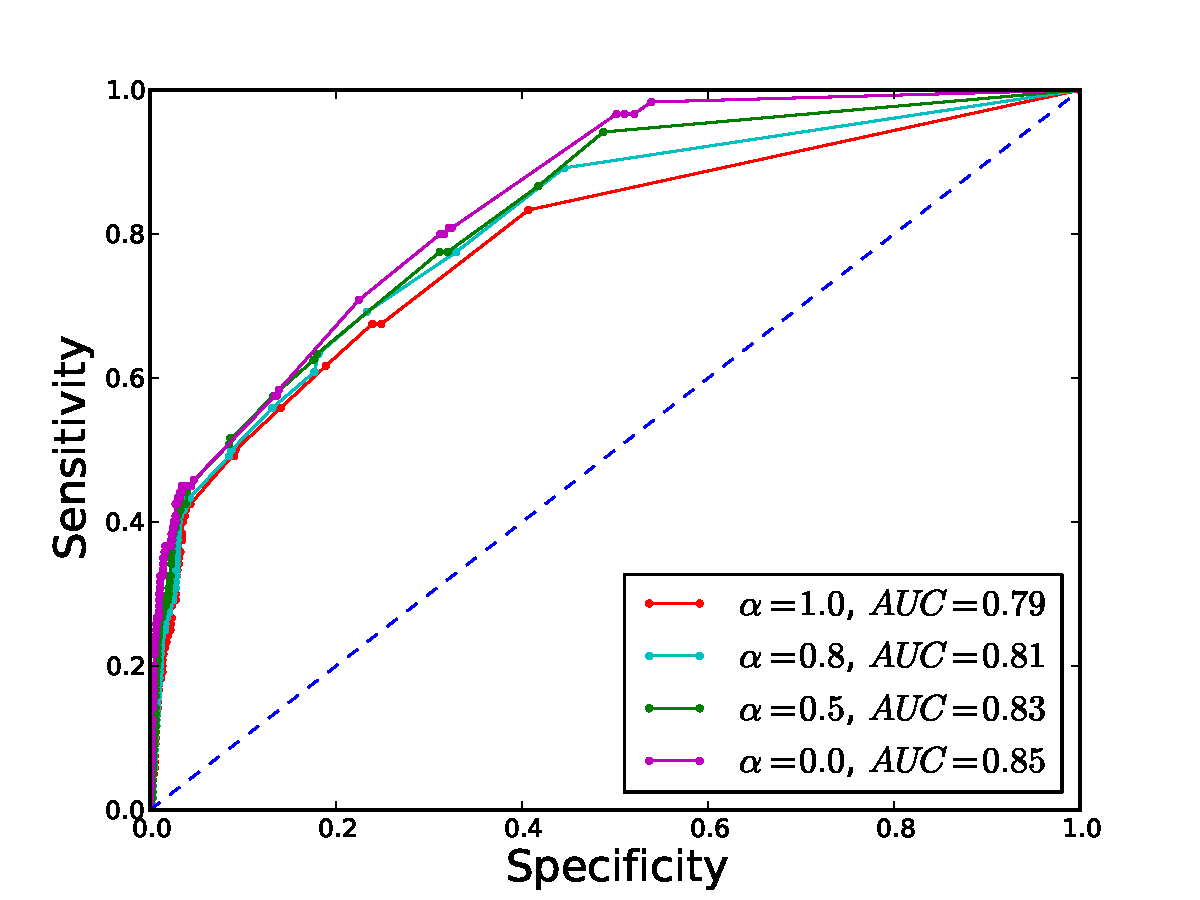
\includegraphics[width=1.2\textwidth]{figures/ROC_6.pdf}
\caption{6 mutations}
\label{fig:ROC6mut}
\end{subfigure}
\hfill
\begin{subfigure}[b]{0.3\textwidth}
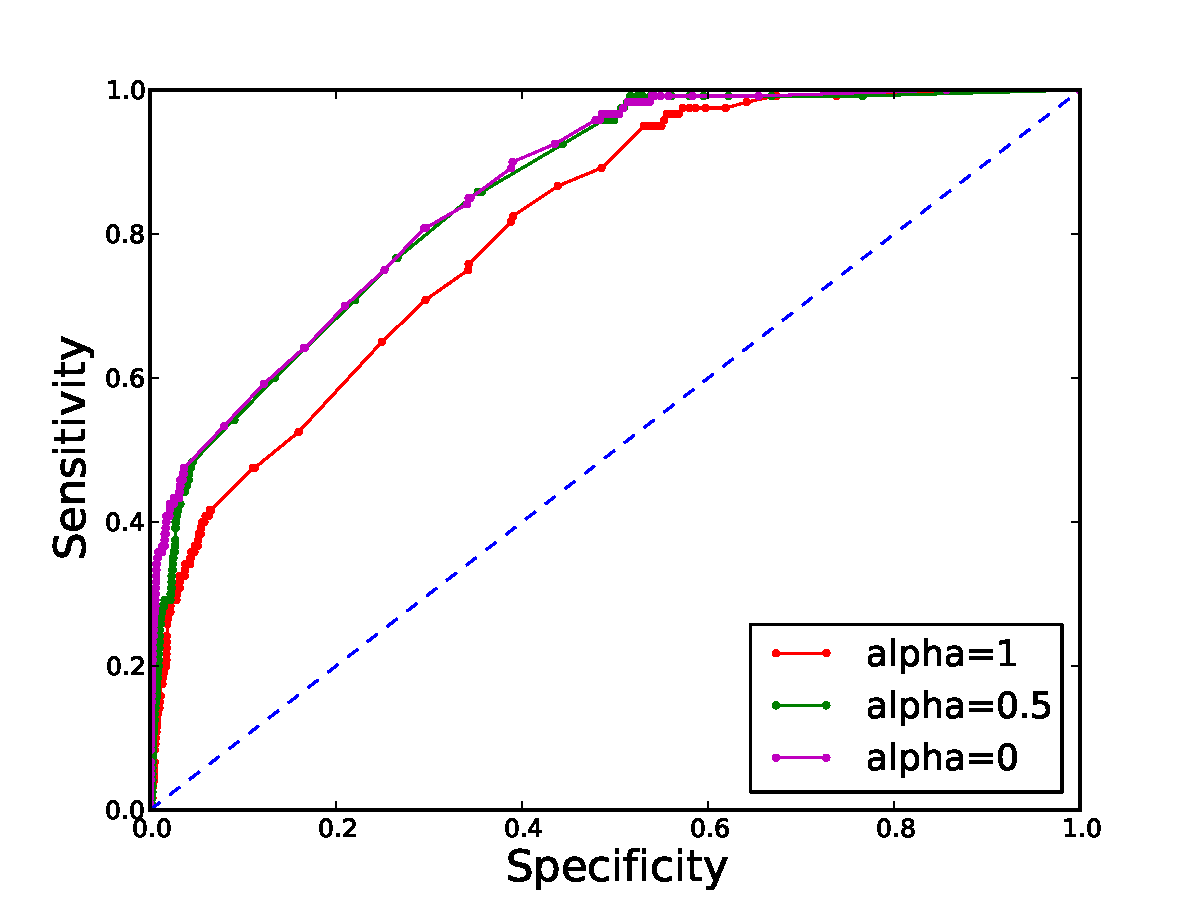
\includegraphics[width=1.2\textwidth]{figures/ROC_12.pdf}
\caption{12 mutations}
\label{fig:ROC12mut}
\end{subfigure}
\hfill
\begin{subfigure}[b]{0.3\textwidth}
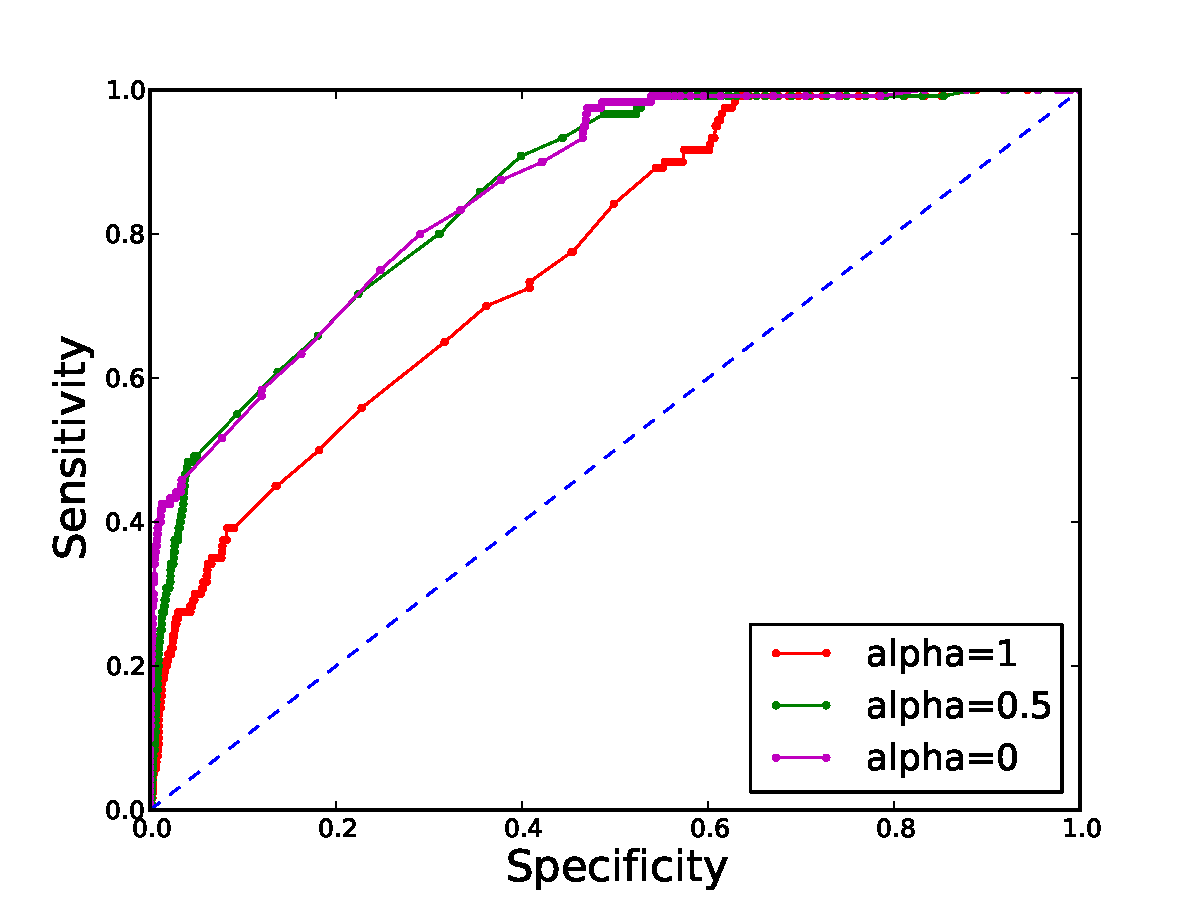
\includegraphics[width=1.2\textwidth]{figures/ROC_24.pdf}
\caption{24 mutations}
\label{fig:ROC24mut}
\end{subfigure}
\caption{Performance of error-correction. Subfigures accuracy with under-estimated error rate (6 mutations), exact estimates (12 mutations) and over estimates 
(24 mutations). We also analyze the impact of the parameter $\alpha$ distributing the weights of stacking pair energies vs isostericity scores and use values 
ranging of $\alpha=\{0,0.5,0.8,1.0\}$. The AUC is indicated in the legend of the figures. Each individual ROC curve represent the average performance over the 10 experiments.}
\label{fig:ROCall}
\end{figure}

Our data demonstrate that our algorithm exhibits interesting performance for error-correction applications. First, the AUC values (up to $0.86$) indicate that a
signal has been successfully extracted. This result has been achieved with errors in loop regions (i.e. without base pairing information) and thus suggests
that correction rates in structured regions (i.e. base paired regions) could be even higher. Next, the optimal values of $\alpha$ tend to be close to $0.0$. This 
finding suggests that at this point the information issued from the stacking energy is currently modest. However, specific examples showed improved performance
using this energy term. Further studies must be conducted to understand how to make the best use it. Finally, our algorithm seems robust to the number of
mutations considered. Indeed, good AUC values are achieved with low estimates of the number of errors in the sequence (c.f. 50\% of the errors  in
Fig.~\ref{fig:ROC6mut}) and with large  values (c.f.~200\% of the errors  in Fig.~\ref{fig:ROC24mut}). It is worth noting that scoring scheme with larger weight on
the isostericity scores (low $\alpha$ values) seem more robust to under- and over-estimate of the number of errors.






%!TEX root = main_RECOMB.tex
\section{Conclusion}
\label{sec:conclusion}

In this article we presented a new and efficient way of
exploring the mutational landscape of an RNA, benefiting from the
 conserved consensus secondary structures  information,
to identify and fix sequencing errors. We also showed a new
 pseudo energy model, taking into account the nearest-neighbour energy model 
and, to quantify geometrical differences,  the isostericity of all base pairs. 

By combining those two approaches,  the 
mutational landscape exploration and the pseudo energy model,
 into \texttt{RNApyro}, we show that we can
correct randomly mutated 5s rRNA sequences. 
As presented in Sec.~\ref{sec:results},
we observe that the models
with larger weights on the
isostericity seems to hold a higher accuracy on the estimation of errors.
Importantly, the implementation is fast enough for practical applications.

We must point out that our approach can only detect point wise 
sequencing errors, and only if they are located in base pairs. It 
nonetheless supplements well existing tools by using previously discarded
information.



%!TEX root = main_RECOMB.tex
\section{Acknowledgments}
\label{sec:acknowledgments}
The authors would like to thank Rob Knight for his suggestions and comments.

\newpage

\bibliographystyle{plainnat}
\bibliography{RNApyro}


\end{document}  
